% 
% ======================================================================
\RequirePackage{docswitch}
% \flag is set by the user, through the makefile:
%    make note
%    make apj
% etc.
\setjournal{\flag}

\documentclass[\docopts]{\docclass}

% You could also define the document class directly
%\documentclass[]{emulateapj}

% Custom commands from LSST DESC, see texmf/styles/lsstdesc_macros.sty
\usepackage{lsstdesc_macros}
\usepackage[utf8]{inputenc}
\usepackage{graphicx}
\usepackage{subfigure}
\graphicspath{{./}{./figures/}}
\bibliographystyle{apj}

% Add your own macros here:


% 
% ======================================================================

\begin{document}

\title{ Impact of the calibration on the performances of the LSST SN survey }

\maketitlepre

\begin{abstract}
We study the impact of the calibration uncertainties, parametrized on one side as random errors in the zeropoint of each filter ($\delta_{zp}$'s) and on the other as shifts in wavelength of each filter ($\delta_\lambda$'s), on the accuracy of the cosmological constraints that will be extracted from LSST SN survey.
We perform a set of simulations of a typical LSST SNe Ia survey.
The standardization of the SNe Ia, their spectrophotometric evolution, the cosmology and the calibration parameters are fitted at the same time to capture all possible interactions between the parameters.
We show that, when all parameters are left free, a nearly complete degeneracy remains between zero points and cosmology, so that accurate external constraints on the flux scale is required. We show that an accuracy of the zeropoint determination better than $1\mathrm{mmag}$ is required to extract most of the statistical information LSST will bring. In the same way we show that an accuracy of the filter mean positions below the $\mathrm{\AA}$ level is required.
\end{abstract}

% Keywords are ignored in the LSST DESC Note style:
\dockeys{photometry: calibration}

\maketitlepost

% ----------------------------------------------------------------------
% 

\section{Introduction}
\label{sec:intro}

Our current knowledge of the dark energy is constrained by the SN Ia surveys and their analysis, the most recent and best constraints come from the analysis of the SN light curves from the Pantheon Sample (\cite{1710.00845}).
It gives the most precise measurement of dark energy to date with $w = -1.031 \pm 0.040$ in a $w\text{CDM}$ model and $w_0 = -1.011 \pm 0.087$ and $w_a = -0.215 \pm 0.402$ for the $w_0w_a\text{CDM}$ model.

While these uncertainties are dominated by the statistics, uncertainty on the photometric calibrration of the SNe Ia remains one important source of systematics as it scales to 5 $\mathrm{mmag}$ over 7000$\mathrm{\AA}$.

With LSST, the statistics will increase by a factor between 10 and 30, putting again stringent constraints on calibration accuracy.

In this context the goal of this work is to study the impact of the calibration uncertainties on the performances of a LSST-like survey, composed of a wide and a deep layer.
We simulate a typical LSST SNe Ia dataset using the light-weight simulation framework \code{SnSim} (DESC note in prep.) and fit a model including the standardization parameters, their spectrophotometric evolution, the cosmology and the calibration parameters at the same time to the simulated data. The performances are evaluated by computing the Figure of Merit (FoM) as a function of a priori knowledge on the calibration parameters.

In section \ref{sec::simulated_dataset} we describe the observing conditions we use in this forecast work to generate the SN Ia light curves and we check their quality.
We present our analysis model for the simulated dataset and the way we handle the calibration uncertainties in §\ref{sec::analysis_model}.
We present our results concerning the performances of the survey for different calibration strategies in section §\ref{sec::results}.
In §\ref{sec::discussion} we discuss the results and we conclude concerning the calibration minimal specifications in §\ref{sec::conclusions}.

% ----------------------------------------------------------------------

\section{Simulated dataset}
\label{sec::simulated_dataset}

\subsection{Cadence}
\label{subsec::cadence}

We assume that the LSST SN survey will be split in two layers:
\begin{itemize}
\item A Wide Fast Deep (WFD) that will be composed of short exposures ($2 \times 15\mathrm{s}$) over a large fraction of the sky using a rolling cadence as currently studied within DESC and LSST Project ( SNWG \& Cadence Task Force).
  This survey will allow to discover a large number of nearby SNe Ia ($z < 0.4$).
\item A Deep Drilling Field  (DDF) survey in which a smaller number of fields will be observed but with longer visits ($\approx \mathrm{600s}$) to provide distant SNe Ia ($ 0.1 < z < 1$).
\end{itemize}

The cadence that will be implemented for the wide and the deep surveys is still in discussion.
For this work we have adopted two nominated scenarii, taken from the current proposed cadences (see Tables \ref{tab:nominal_scenario_wide} \& \ref{tab:nominal_scenario_DDF}).
The goal of this work is to evaluate the impact of calibration systematics on the cosmological measurements, performed with SNe and not to study the impact of the effective cadence and observing conditions.
For this reason, we have deliberately simplified the light-curve generation by defining an average cadence in each filter.
This average cadence corresponds to what is delivered by the \code{Altsched} \& \code{Altsched-rolling} nominal requirements for well sampled light-curves. We expect a total of 2000 spectroscopically confirmed SNe Ia per year in the wide component and 1500 in the deep one.

\begin{table*}[t]
\begin{center}
  \caption{Nominal scenarii for the wide that allows to build a SN
    sample complete up to $z \sim 0.4$. The two cadences given in each
    column are for the rolling/standard cadences.}
\label{tab:nominal_scenario_wide}
\begin{tabular}{l|cccc}
\hline
\hline
              & $g$ & $r$ & $i$ & $z$ \\
\hline 
$T_{exp}$      & 30       &   30    &  30        & 30  \\
$m_{5\sigma}$ (per visit)  &  24.83   &  24.35   &  23.88    &  23.30  \\
cadence [days]       & 7.7 / 13.6 & 2.9 / 5.6 & 4.3 / 8.2 & 3.3 / 6.7  \\
%Target amplitude SNR & $>30$ & $>40$ & $>30$ & $>20$ \\
\hline
\end{tabular}
\end{center}
\end{table*}

\begin{table*}[t]
\begin{center}
\caption{A nominal scenario for the DDF that allows to build a SN
  sample complete up to $z \sim 0.75$.}
\label{tab:nominal_scenario_DDF}
\begin{tabular}{l|cccc}
\hline
\hline
              & $r$ & $i$ & $z$ & $y$ \\
\hline 
$T_{exp}$      & 600 & 600 & 720 & 600 \\
$m_{5\sigma}$ (per visit)  & 26.05 & 25.56 & 25.06 & 24.08 \\
cadence  [days]     &  \multicolumn{4}{c}{5 days} \\
%Target amplitude SNR & $>25$ & $>60$ & $>35$ & $>20$ \\
\hline
\end{tabular}
\end{center}
\end{table*}

We build our forecast upon those two nominal scenarii, assuming respectively 30s and 1800s exporures in 4 bands with a regular cadence of 3 days and without loss due to weather. Exact numbers are given in Table \ref{tab:nominal_scenario_wide}  and \ref{tab:nominal_scenario_DDF}. This study will be updated as work on the rolling cadence progresses.

\subsection{Instrument Model and Observing conditions}

We use the most recent model from \cite{SMTN-002} (SMTN-002). The previous model, described in \cite{LSE-40} (LSE-40) has been revised and the new troughput is 40\% lower  in SMTN-002.
We use median observing conditions (same for all epoch) for each filter in Figure \ref{fig:zp}.

\begin{figure}[t]
\begin{center}
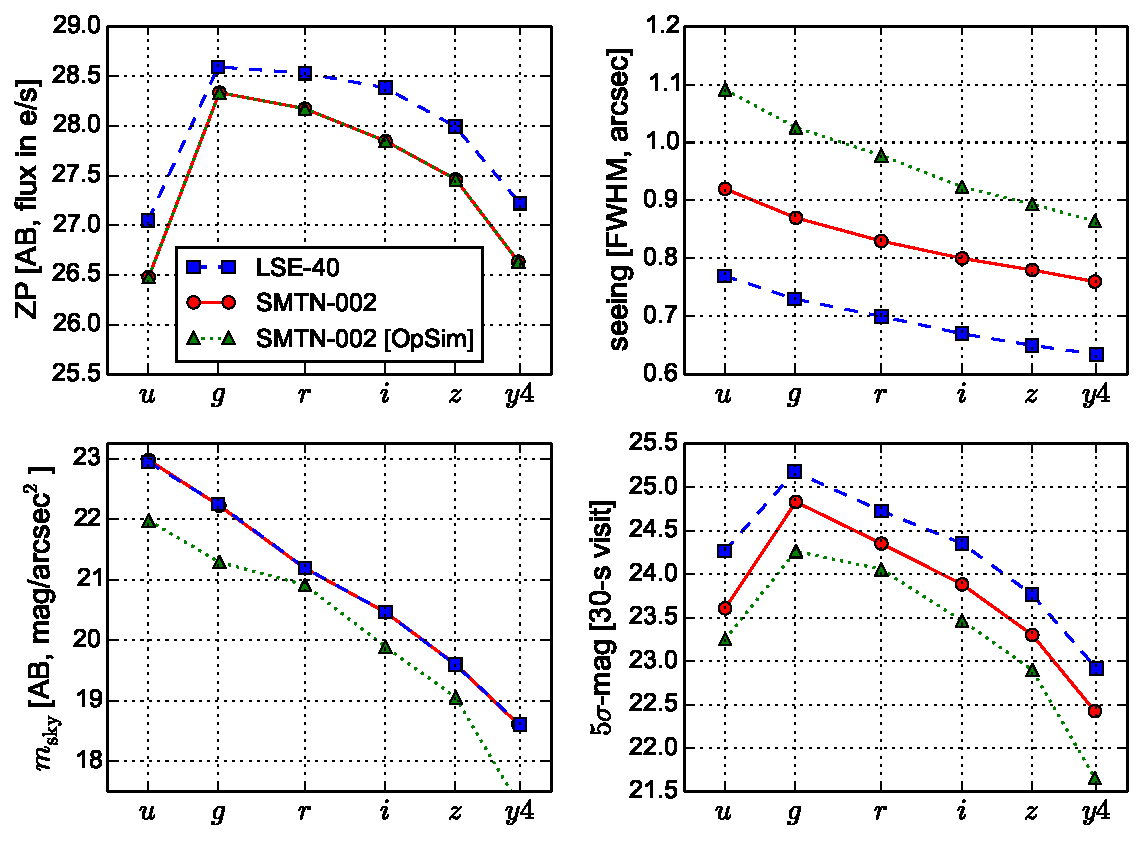
\includegraphics[width=\linewidth]{lsst_model_summary.pdf}
\caption{Parameters of the survey simulation : from left to right and top to bottom we have : zero-points, median seeing, brightness of the background sky (dark time) and survey limiting magnitudes, this Figure is reproduced from \cite{SN-CADENCE} in each $grizy$ band.}
\label{fig:zp}
\end{center}
\end{figure}

\subsection{Simulated SNe}
\label{ssec::snsim}
We use \code{SnSim} (DESC note in prep.) to produce the observed SNe Ia and their light curves with the cadence and observing conditions detailed in the previous parts.
Our study is performed for 1, 5 and 10 years of the LSST SN-survey.
The distribution in redshift of the simulated SNe Ia is shown in Figure \ref{fig:z_distrib}.

\begin{figure}[ht]
  \centering
  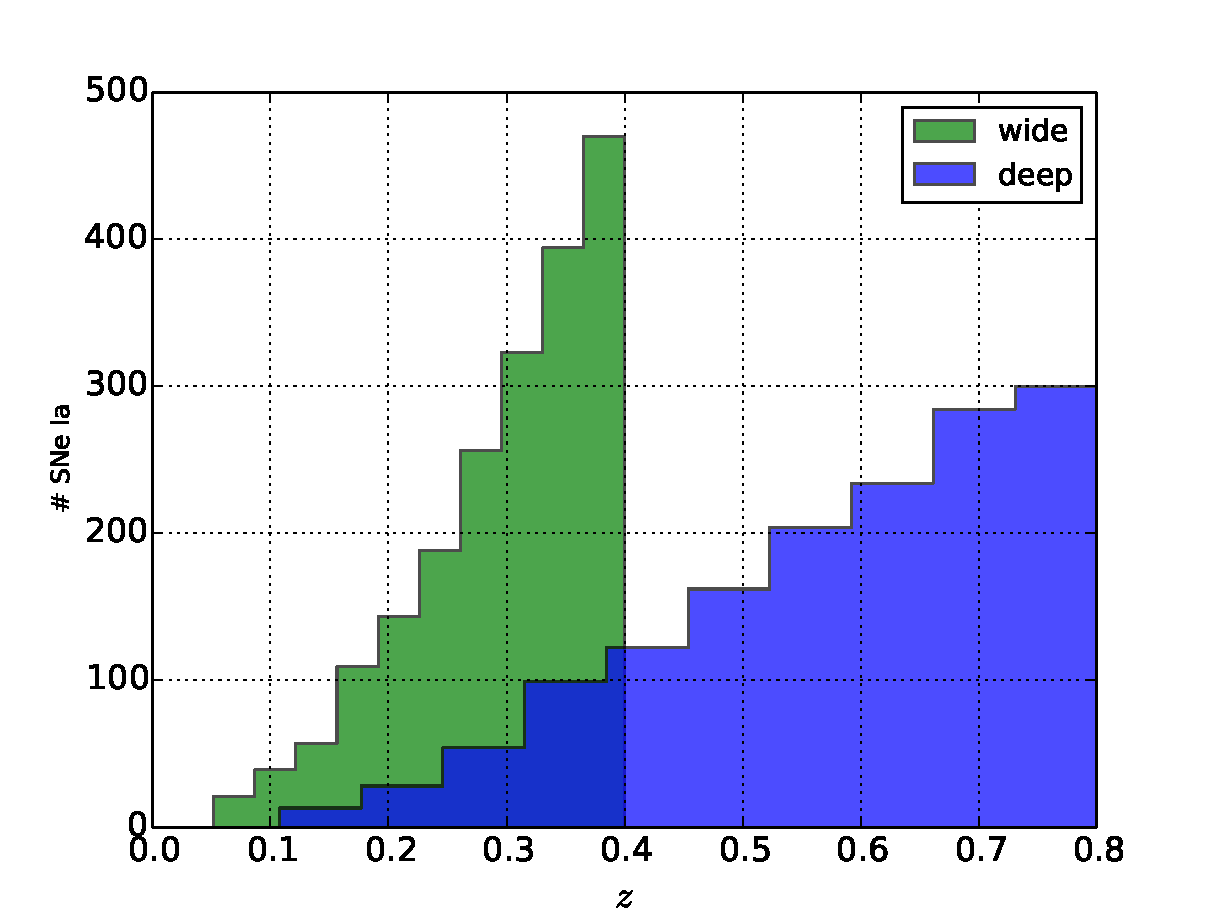
\includegraphics[width=\linewidth]{redshift_distribution_one_season.pdf}
  \caption{Redshift distribution of the SNe Ia simulated with one year of wide and deep layers for a total of $\approx 3.5\times10^3$ SNe Ia.}
  \label{fig:z_distrib}
\end{figure}
In Figure \ref{fig:lc_examples} we show that in two extreme cases of SNe Ia, one from the wide layer at $z=0.06$ and one from the deep layer at $z=0.87$, the light curves we obtain are well sampled in time and the uncertainty associated to each flux measurement is reasonably low compared to the light curve amplitude..

\begin{figure*}[t]
\begin{center}
\subfigure[$z = 0.15$]{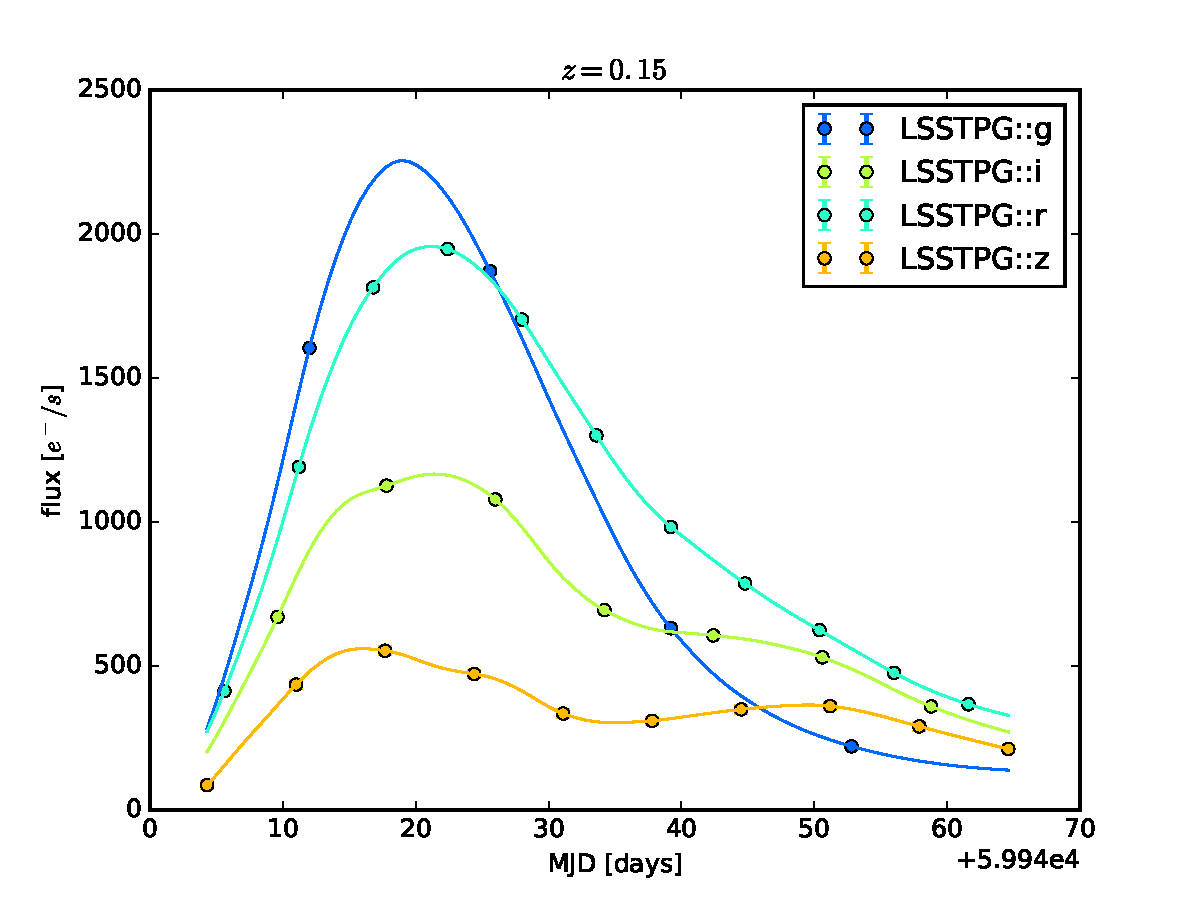
\includegraphics[width=0.48\linewidth]{sn-lc_wide-AltSched_z015.pdf}}
\subfigure[$z = 0.71$]{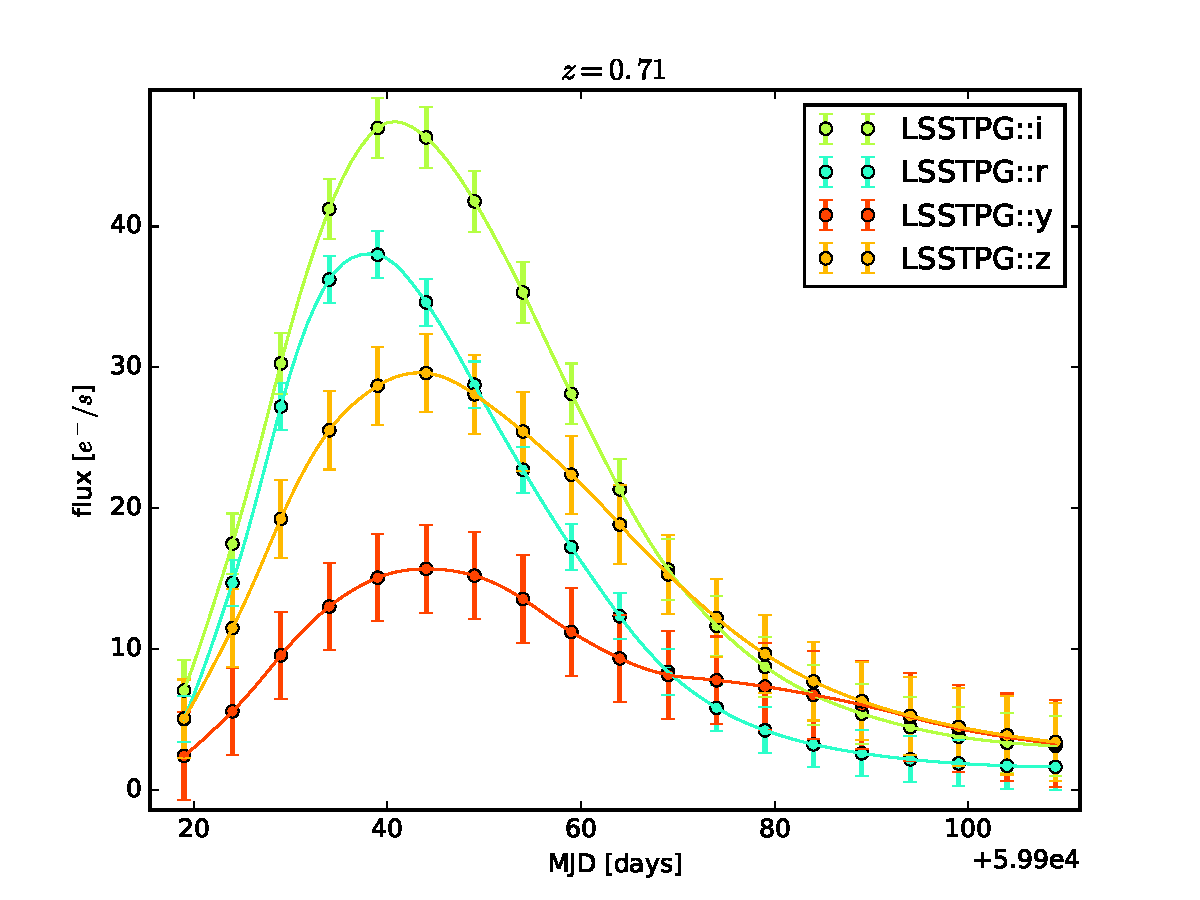
\includegraphics[width=0.48\linewidth]{sn-lc_deep_z071.pdf}}\\
\caption{Light curves for a SN Ia measured in the wide layer at $z=0.15$ in $griz$ bands (left) and a SN Ia measured in the deep layer at $z=0.71$ in $rizy$ bands (right).}
\label{fig:lc_examples}
\end{center}
\end{figure*}

Finally, we show in Figure \ref{fig:sigmas} that in each layer the color $c$, the time of maximum luminosity $t_0$ and the stretch of the simulated SNe Ia are well measured over the entire redshift range in both survey layers.

\begin{figure*}[t]
\begin{center}
\subfigure[wide]{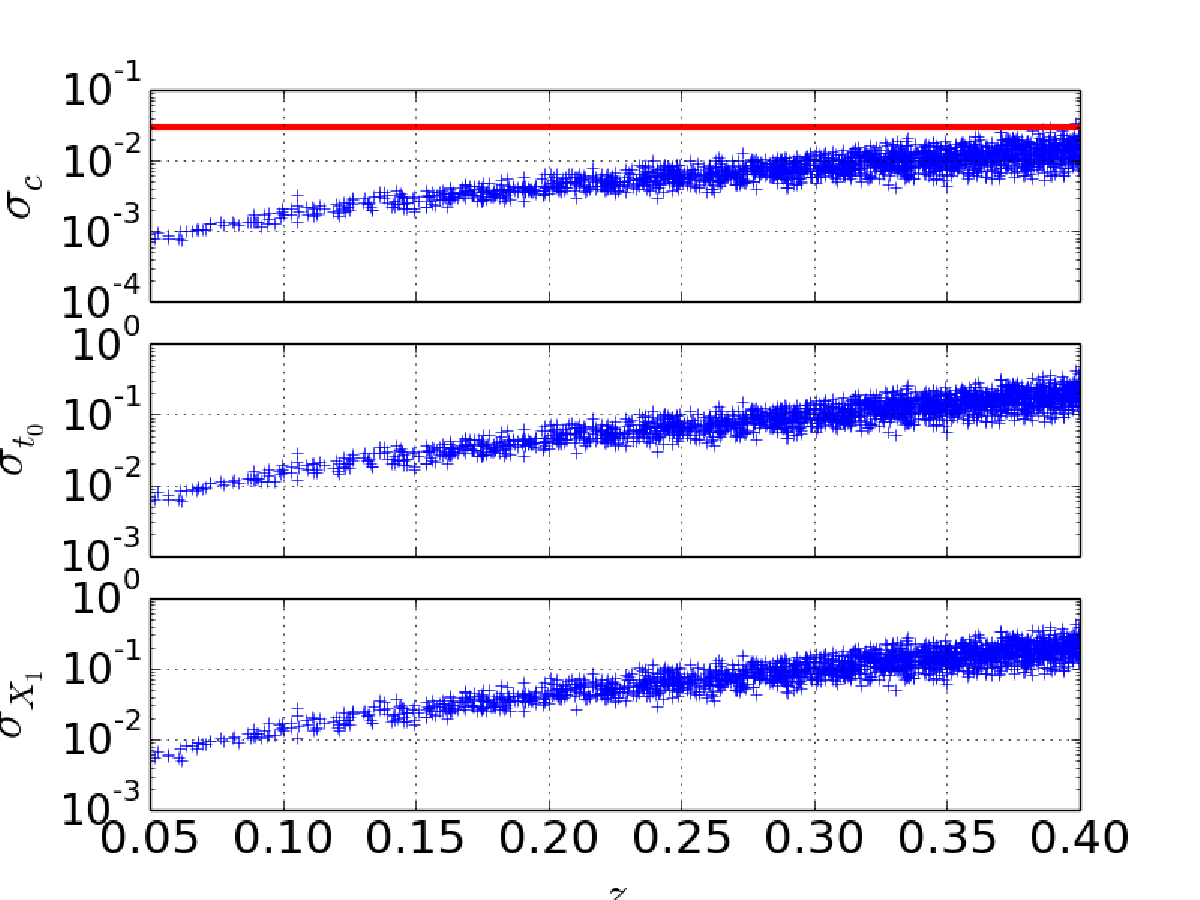
\includegraphics[width=0.48\linewidth]{lsst_wide_WFC_sigmas_2000SNe.pdf}}
\subfigure[deep]{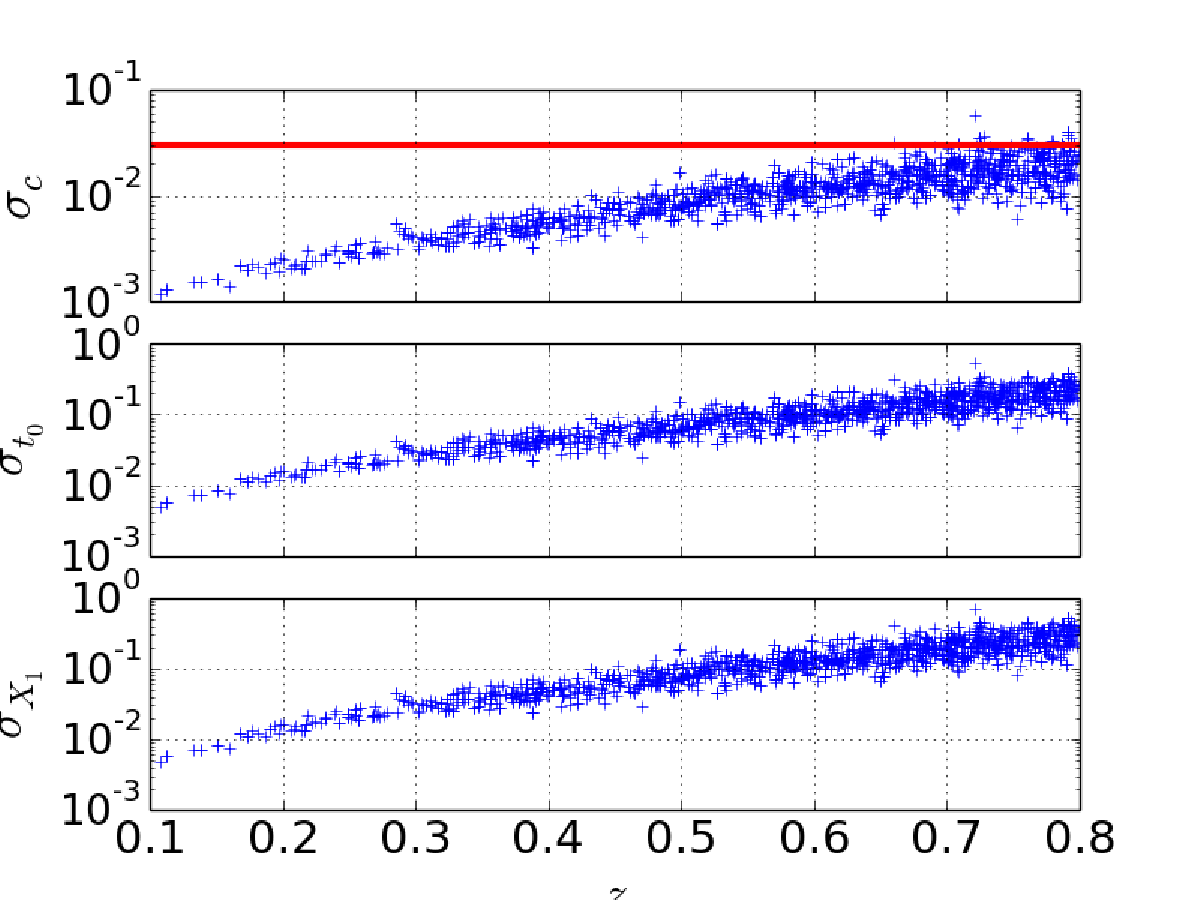
\includegraphics[width=0.48\linewidth]{lsst_deep_DDF_sigmas_1500SNe.pdf}}\\
\caption{Uncertainty of the color, the time of maximum luminosity and the stretch of each SN Ia (from top to bottom) in the wide (left) and the deep (right) layers. The horizontal red line corresponds to $\sigma_c = 0.03$ which is the threshold on the accuracy on the color of a well measured SN Ia}
\label{fig:sigmas}
\end{center}
\end{figure*}

% ----------------------------------------------------------------------

\section{Analysis Model}
\label{sec::analysis_model}

We now describe how we evaluate the analysis of the SNe Ia data as it is likely to be performed in 2020+, we have developed a small pipeline that implements : (1) Light curves fit, (2) training of a spectrophotometric model, (3) standardization of the SNe Ia and (4) a cosmology. 

\subsection{Model details}
\label{subsec::model_details}
We want our model to be representative of a real analysis, while avoiding the complexity and numerical clumsiness of a complete spectroscopic model.
In order to avoid the need of including spectra in our simulation, we will mimick their effect on broadband quantities.
The calibration uncertainties induce redshift dependent errors on magnitude and color.
It is thus of primary importance to account for all the spectral effects in order to accurately propagate calibration uncertainties.
On the contrary, the SN light-curve shape (stretch) is expected to be well constrained thanks to the good sampling (\ref{ssec::snsim}), and calibration uncertainties do not strongly impact shapes (e.g. \cite{1401.4064} Figure 6).
We thus choose to skip the time dependant part, only modeling the flux of each measured SN Ia in each used band, interpolated at the day of maximum luminosity in the restframe $B$ band (hereafter DayMax).
The flux of a given SN Ia measured at DayMax in a band $b$ (in $\mathrm{e^{-}/s/cm^2}$) can be modeled as follows:

\begin{equation}
\label{eq::flux_model}
\varphi_b = \frac{1}{1+z} \times \frac{10^{-10}}{d_L^2(z, \theta_\text{c})}\times \int \frac{10^{-10}\lambda}{hc} S\left(\frac{\lambda}{1+z}\right) T_b(\lambda) d\lambda \text{ ,}
\end{equation}
where $z$ and $d_L$ are respectively the redshift and the luminosity distance (in $\mathrm{Mpc}$) of the given supernova,
$\theta_\text{c}$ is the vector of the cosmological parameters (depending on the model we choose to use),
$S\left(\frac{\lambda}{1+z}\right)$ is the SED of a standard SN Ia (in $\mathrm{erg/s/\AA/cm^2}$) at 10 $\mathrm{pc}$ and $T_b(\lambda)$ is the transmission of the detector in a band $b$ (in $\mathrm{e^-/phot}$).
Translating equation \ref{eq::flux_model} into magnitudes:
\begin{equation}
\begin{split}
\label{eq::raw_model}
m_b = &\mu(z, \theta_\text{c}) + 25 + 2.5\log_{10}(1+z) \\
&- 2.5\log_{10}\int \frac{10^{-10}\lambda}{hc} S\left(\frac{\lambda}{1+z}\right) T_b(\lambda) d\lambda \text{ ,}
\end{split}
\end{equation}
where $\mu(z, \theta_\text{c})$ is its distance modulus related to the luminosity distance $d_L$ as $\mu(z, \theta_\text{c}) = 5\log_{10}(d_L)$.

Then we perform a polynomial expansion around the central wavelength of the passband $\bar\lambda_b$.
Since we work only with photometric data, we perform a linear approximation of the spectrum over a range centered on the mean wavelength of the passband $\bar\lambda_b$.
We have then:

\begin{equation}
\int \lambda S\left(\frac{\lambda}{1+z}\right) T_b(\lambda) d\lambda \approx \bar{S}(\frac{\bar\lambda_b }{1+z}) \times \int \lambda T_b(\lambda) d\lambda
\end{equation}
where $\bar{S}(\frac{\bar\lambda_b }{1+z})$ is the mean of the spectrum over the considered passband.
$\bar\lambda_b$ evaluated as $\bar\lambda_b = \frac{\int \lambda^2 T_b(\lambda) d\lambda}{\int \lambda T_b(\lambda) d\lambda}$ for the term of $1^{st}$ order to vanish in the integral.

Our model in eq \ref{eq::raw_model} becomes:          
\begin{equation}
  m_b = \mu(z, \theta_\text{c}) + 25 + 2.5\log_{10}(1+z) - 2.5 \log_{10} \bar{S}(\bar\lambda_b ) + \mathcal{Z}_b \text{ ,}
\end{equation}
where $\mathcal{Z}_b = -2.5 \log \int \frac{10^{-10}\lambda}{hc} T_b(\lambda) d\lambda$ is the band zeropoint.

As we will show later, care must be taken while modeling the SED of the supernovae and its characterization shall remain free to evolve with the input data.
We decompose $-2.5\log_{10}\bar{S}(\bar\lambda_b)$ on 4 different terms:
\begin{equation}
-2.5\log_{10}S(\bar\lambda_b) = M_X + P(\frac{\bar\lambda_b}{1+z}) + cQ(\frac{\bar\lambda_b}{1+z}) + c\beta \text{ ,}
\end{equation}
where $P(\frac{\bar\lambda_b}{1+z})$ plays the role of the mean restframe spectrum of a "standard" SN Ia, $M_X$ is a normalization factor accounting for the restframe absolute luminosity of each SN, $Q(\frac{\bar\lambda_b}{1+z})$ is a color law accounting for the color variation of each SN around the mean SN spectrum and $\beta$ is the brighter-bluer parameter that relates flux variation to SNe color.
We also introduce here the color $c$ of each SN.
We decompose the mean spectrum over a B-spline basis of degree 2, and the color law over a polynomial of fourth degree.

$\beta$ plays the role of the degree 0 in $Q( \lambda )$. We fix it in $Q( \lambda )$ by imposing $Q(\lambda_B) = 0$ and $Q(\lambda_V) = -1$, $\lambda_B$ and $\lambda_V$ being respectively the $B$ and $V$ band mean wavelengths.

Incorporated to the model it gives:

\begin{equation}
\begin{split}
\label{eq::model}
m_b = &M_X + 25 + \mu(z, \theta_\text{c}) + 2.5\log_{10}(1+z) \\
&+ P(\frac{\bar\lambda_b }{1+z}) + cQ(\frac{\bar\lambda_b }{1+z}) + c\beta + \mathcal{Z}_b \text{ .}
\end{split}
\end{equation}

At this stage other degeneracies appear between these different parameters.
The way to handle these degeneracies is to add priors to our model.
If $J$ is the matrix of the derivatives  of our model with respect to all free parameters (columns) for all light curve amplitudes measured (lines), we can vertically add matrices to $J$ for each prior, corresponding to one or more "additionnal" measurements:
\begin{equation}
J =
\begin{pmatrix}
  J \\
  J_\text{priors}
\end{pmatrix} 
\end{equation}

In parallel, if $C$ is the covariance matrix of our measurements, we add diagonally the covariance matrix of the prior to $C$:
\begin{equation}
C =
\begin{pmatrix}
  C & 0 \\
  0 & C_\text{priors}
\end{pmatrix} \text{ .} 
\end{equation}

In our case we add the following priors:
\begin{itemize}
\item The spectrum normalization, to cut degeneracy with the distance modulus $\mu$ that could increase while $M_X$ decrease.
\item The spectrum color, that is degenerated with the color law.
\item The fact that the color law is fixed at $\lambda_B$ to 0 and at $\lambda_V$ to -1 (shown above).
\item We fix all the $M_X$'s at a same value to cut degeneracies with the distance moduli but with a dispersion of 14\% to account for the intrinsic dispersion of the SNe Ia absolute maximum luminosity.
\item Since we use a $w_0w_a$ cosmology, $\theta_\text{c} = \{ \Omega_m$, $\Omega_k$, $w_0$, $w_a$, $H_0$, $\Omega_bh^2 \}$, we add a Planck prior from \cite{1502.01589}, which brings us the information on $H_0$ and $\Omega_k$ we would not get with the SNe Ia only.
\end{itemize}

% ----------------------------------------------------------------------

\subsection{Calibration parameters}
\label{subsec::calib_uncertainties}
The core of this work is about the way we handle the calibration errors and incorporate them in \ref{eq::model}.
We describe them with two different parameter subsets:
\begin{itemize}
\item $\delta zp$'s, that takes into account the error we make on the normalization of the transmission in each band.
There is one associated to each filter we use.
\item $\delta \lambda$'s, which is the error made in observer frame on the mean wavelength position of each filter. 
\end{itemize}

Our model finally becomes :
\begin{equation}
\begin{split}
m_b = & M_X + 25 + \mu(z, \theta_\text{c}) + 2.5\log_{10}(1+z) + \mathcal{Z}_b \\
&+ P(\frac{\bar\lambda_b  + \textcolor{red}{\delta\lambda_b}}{1+z}) + cQ(\frac{\bar\lambda_b  + \textcolor{red}{\delta\lambda_b}}{1+z}) + {c\beta} + \textcolor{red}{\delta zp_b} \text{ .}
\end{split}
\end{equation}

\subsection{Structure of the Calibration covariance matrix}
\label{subsec::covmat}
These calibration parameters are associated to a calibration covariance matrix $C_s$.
The structure of $C_s$ depends on the calibration strategy. In particular it is generally non diagonal because of the interplay between $zp$ and filter positions.
The state of the art concerning SNe Ia flux measurements consists in comparing their flux directly with calibrated astrophysical standards.
We suppose that the zeropoint of a band $b$ is obtained using the flux measurement of this calibrated astrophysical standard, which is modeled as:
\begin{equation}
zp_b = \int T_b(\lambda) S_{std}(\lambda) d\lambda + n_b \text{ ,}
\end{equation}
where $T$ is the transmission of the instrument, $S_{std}$ is the spectrum of the astrophysical standard and $n_b$ is a random noise with $cov(n_b) = \sigma_{zp_b}^2$.
This way of measuring flux leads to the fact that if we make an error on the wavelength position of the filters, the flux integration of the standard will not be what we should expect and thus leads to an error on the zeropoint of the band.
In fact we have:
\begin{equation}
\begin{split}
zp_b &= \int \bar T_b(\lambda) S_{std}(\lambda) d\lambda + n_b + \frac{\partial \int{T_b(\lambda)S(\lambda)d\lambda}}{\partial \bar\lambda_b }\\
&= \bar{zp}_b + e_{zp_b} + \frac{\partial zp_b}{\partial \bar\lambda_b }\delta\bar\lambda_b 
\end{split}
\end{equation}
We then have:
\begin{equation}
\begin{pmatrix}
  zp \\
  \bar\lambda_b 
\end{pmatrix}
=
\begin{pmatrix}
  1 & \frac{\partial zp}{\partial \lambda} \\
  0 & 1
\end{pmatrix}
\begin{pmatrix}
  e_{zp} \\
  \delta\bar\lambda_b 
\end{pmatrix}
+
\begin{pmatrix}
  \bar{zp} \\
  0
\end{pmatrix}
\end{equation}
We define $\frac{\partial zp}{\partial \lambda}$ as the change in zeropoint for $1 \mathrm{\AA}$ of filter position error, obtained by comparing the integrated flux of an astrophysical standard (P330E in this case) in a reference filter and in a shifted filter.
We have:
\begin{equation}
C_s = cov
\begin{pmatrix}
  zp \\
  \bar\lambda_b 
\end{pmatrix}
=
\begin{pmatrix}
  1 & \frac{\partial zp}{\partial \lambda} \\
  0 & 1
\end{pmatrix}
\begin{pmatrix}
  \sigma_{zp}^2 & 0 \\
  0 & \sigma_{\lambda}^2
\end{pmatrix}
\begin{pmatrix}
  1 & 0 \\
  \frac{\partial zp}{\partial \lambda} & 1
\end{pmatrix}\text{ .}
\end{equation}
We put the values in Table \ref{tab::calib_derivatives}, then $C_s$ becomes :
\begin{equation}
\label{eq::cov_calib}
C_s = 
\left( \begin{array}{cc|cc} \sigma^2_{ zp_{g}} + (\sigma_{\lambda_g} \frac{\partial zp_g}{\partial \lambda_g})^2 & 0 & \frac{\partial zp_g}{\partial \lambda_g} \sigma^2_{ \lambda_g} & 0 \\ 0 & \ddots & 0 & \ddots \\ \hline \frac{\partial zp_g}{\partial \lambda_g} \sigma^2_{ \lambda_g} & 0 & \sigma^2_{\lambda_{g}} & 0 \\ 0 & \ddots & 0 & \ddots \end{array} \right) \text{ .}
\end{equation}

\begin{table*}[t]
\begin{center}
\caption{$\delta zp$'s derivatives with $\delta\lambda$'s computed using P330E spectrum.}
\label{tab::calib_derivatives}
\begin{tabular}{l|ccccc}
\hline
\hline
  & $g$ & $r$ & $i$ & $z$ & $y$ \\
\hline 
  $\frac{\partial\delta zp}{\partial\delta \lambda}$ $[\mathrm{mmag/\AA}]$& 0.026 & 0.18 & 0.24 & 0.23 & 0.22\\
\hline
\end{tabular}
\end{center}
\end{table*}

% ----------------------------------------------------------------------

% \subsection{Model degeneracies}
% \label{ssec::model_deg}

% At this current stage our model have some degeneracies that we must get rid of.
% The way to handle this degeneracies is to add priors to our model.
% If $J$ is the matrix of the derivatives  of our model with respect to all free parameters (columns) for all light curve amplitudes measured (lines), we can vertically add matrices to $J$ for each prior, corresponding to one or more "additionnal" measurements:
% \begin{equation}
% J =
% \begin{pmatrix}
%   J \\
%   J_\text{priors}
% \end{pmatrix} 
% \end{equation}

% In parallel, if $C$ is the covariance matrix of our measurements, we add diagonally the covariance matrix of the prior to $C$:
% \begin{equation}
% C =
% \begin{pmatrix}
%   C & 0 \\
%   0 & C_\text{priors}
% \end{pmatrix} 
% \end{equation}

% In our case we add the following priors:
% \begin{itemize}
% \item The spectrum normalization, to cut degeneracy with the distance modulus $\mu$ that could increase while $M_X$ decrease.
% \item The spectrum color, that is degenerated with the color law.
% \item The fact that the color law is fixed at $\lambda_B$ and $\lambda_V$ respectively mean wavelength of the $B$ and $V$-bands
% \item We fix the dispersion of the $M_X$'s at 14\% because otherwise we have degeneracies with the distance moduli.
% \item Since we use a $w_0w_a$ cosmology, $\theta_\text{c} = \{ \Omega_m$, $\Omega_k$, $w_0$, $w_a$, $H_0$, $\Omega_bh^2 \}$, we add a Planck prior, extracted from Planck 2015 results(\cite{1502.01589}), which brings us the information on $H_0$ and $\Omega_k$ we wouldn't get with the SNe Ia only.
% \end{itemize}


% ----------------------------------------------------------------------

\subsection{Error propagation}
\label{sec::linalg}

The analysis of a real SN Ia data sample would need us to perform a simultaneous fit marginalized over all Table \ref{tab:params} parameters. Because of the high number of parameters, to ensure a quicker execution and avoid memory issues we work with sparse matrices.

\begin{table*}[t]
\begin{center}
\label{tab:params}
\caption{Summary of our model free parameters}
\begin{tabular}{l|ccccccccc}
\hline
\hline
Free parameters & $M_X$ & $\theta_\text{c}$ & $\theta_P$ & $\theta_Q$ & $c$ & $\beta$ & $\mathcal{Z}$ & $\delta zp$ & $\delta \lambda$ \\
\hline
\# parameters & $N$ & 6 & 31 & 5 & $N$ & 1 & 5 & 5 & 5 \\
\hline
\end{tabular}
\end{center}
\end{table*}

The fit of our model $\mathcal{M}$ would be performed by minimizing the following $\chi^2$:
\begin{equation}
\chi^2 = \sum_{sb}\frac{[m_{sb} - \mathcal{M}(s, b, \vec\theta)]^2}{\sigma_{sb}} \text{ .}
\end{equation}
We suppose that our model is smooth, so we linearize it around the maximum.

Our linearized model $\mathcal{M'}$ describe the data as follows::
\begin{equation}
\mathcal{M'} = J \times \vec\theta
\end{equation}
Where $J$ contains the derivatives of our model with respect to all free parameters (columns) for all light curve amplitude measured (lines) and $\vec\theta$ the vector of all our free parameters (details in Table \ref{tab:params}).

The normal equation for this $\chi^2$ is:
\begin{equation}
J^TC^{-1}J = J^TC^{-1}y
\end{equation}
where $C$ is the covariance matrix of the measurements.

Finally we add the calibration covariance matrix $C_s$ (explicited in §\ref{subsec::calib_uncertainties}) as a prior to our model (as in §\ref{subsec::model_details}).
For the moment we have to keep in mind that these value are not fixed, and we are going to make this study for several examples of what would be the calibration accuracy for the LSST SN survey.

Since we want to study the performances of the survey, we do not need to perform a fit.
In order to get the uncertainties of our model parameters, we compute the Fisher information matrix, that we call $H$, around the best fit.
\begin{equation}
H = J^TWJ
\end{equation}
where $W = C^{-1}$.

According to the Cramér–Rao bound, the inverse of $H$ is a lower bound on the covariance matrix of all our free parameters.

To ensure the consistency of our analysis and the way we propagate the calibration uncertainties, we test our pipeline on the JLA data sample (light curves amplitudes in each band and their SNR).
JLA calibration covariance matrix has the same design as ours, meaning it is composed of the errors on the zeropoints, those on the filter positions, and the corelation terms, for instruments used to obtain the JLA sample.
If we run our pipeline using this calibration covariance matrix and a $\Lambda\text{CDM}$ cosmology, we obtain an uncertainty on $w$ of 5.2\% (stat + sys) when \cite{1401.4064} obtained 5.7\%.
We suppose this difference comes from the fact we are only using SN light curve amplitudes and we can see this only affects the statistical part, as we obtain 3.9\% from the systematics only, it is very close from what was obtained in the JLA analysis, and therefore we suppose that the impact of calibration is well reproduced by our method.

% ----------------------------------------------------------------------

\section{Results}
\label{sec::results}
We study the performances through the Figure of Merit ($FoM$), defined as:
\begin{equation}
FoM = \frac{1}{\sqrt{det(cov(w_0, w_a))}} \text{ .}
\end{equation}
We can then perform a block inversion of $H$.
We modify the calibration strategy by changing the $\sigma_{\delta \lambda}$'s and the $\sigma_{\delta zp}$'s in $C_s$ (eq \ref{eq::cov_calib}) which impact $H$ through $W$.
We compute the $FoM$ with $\sigma_{\delta zp} = \sigma_{zpg} = \sigma_{zpr} = \sigma_{zpi} = \sigma_{zpz} = \sigma_{zpy}$, and $\sigma_{\delta\lambda} = \sigma_{\lambda_g} = \sigma_{\lambda_r} = \sigma_{\lambda_i} = \sigma_{\lambda_z} = \sigma_{\lambda_y}$ at 20 different values from $\sigma_{\delta zp} = 10^{-5}\mathrm{mag}$ to $\sigma_{\delta zp} = 1\mathrm{mag}$ and $\sigma_{\delta \lambda} = 10^{-2}\ \mathrm{\AA}$ to $\sigma_{\delta \lambda} = 100\mathrm{nm}$. We do not observe any difference between the two sets of cadence in the wide layer detailed in \ref{subsec::cadence}. We present these results for one, five and ten years of survey in Figure \ref{fig:fom_grids} for the standard wide cadence

\subsection{Zeropoints}
We can see on this figure that in the three cases, we observe an area at high calibration uncertainties ($\sigma_{zp} > 10\ \mathrm{mmag}$), where the performances of the survey are very low, a plateau at high knowledge on the calibration, where the survey performances are higher and statistics-dominated, and a transition area, where the performances of the survey are equivalently dominated by the statistics and the systematics, it is in this area that given improvements on the calibration lead to the highest shift on the performances.

Concerning the photometric calibration, if we consider that the current uncertainties on the $\delta zp$'s are at $5 \mathrm{mmag}$ (\cite{1401.4064}), we can see that one year of survey with the current zeropoint calibration, we could obtain a $FoM$ of $\approx 30$, while improving it to $1 \mathrm{mmag}$ would allow us to reach a $FoM$ of 60. At 5 years of survey, having a photometric calibration between 1 and 2 $\mathrm{mmag}$ appears to be mandatory to extract at least 50\% of the performances the statistics could grant us. Finally we can see that a calibration below the mmag level should be reached to make use of the full statistics of the LSST SN-survey.

\subsection{Filters}
We observe approximately the same behaviour when looking at the uncertainty on the filter mean position. At one year of survey, we would need the filter mean position uncertainty to be at  $\approx 1\mathrm{nm}$ for for it not to be predominant with respect to the statistics. At 5 years the transition occurs at $2 \mathrm{\AA} < \sigma_{\delta\lambda} < 4 \mathrm{\AA}$ and with the full dataset the filter mean position needs to be below the $\AA$ level. The main difference in behaviour compared to the photometric calibration is that that the FoM seems to reach a non-zero plateau at low accuracy on the filter mean position. It is due to an auto-calibration phenomenon of the uncertainty on $\delta\lambda$, we come back to this in the next session.

Besides these considerations, we can see that the huge ammount of statistics would allow us to get a FoM of 320 at 5 years and 680 at 10 years.

\begin{figure*}[t]
\begin{center}
\subfigure[1 year]{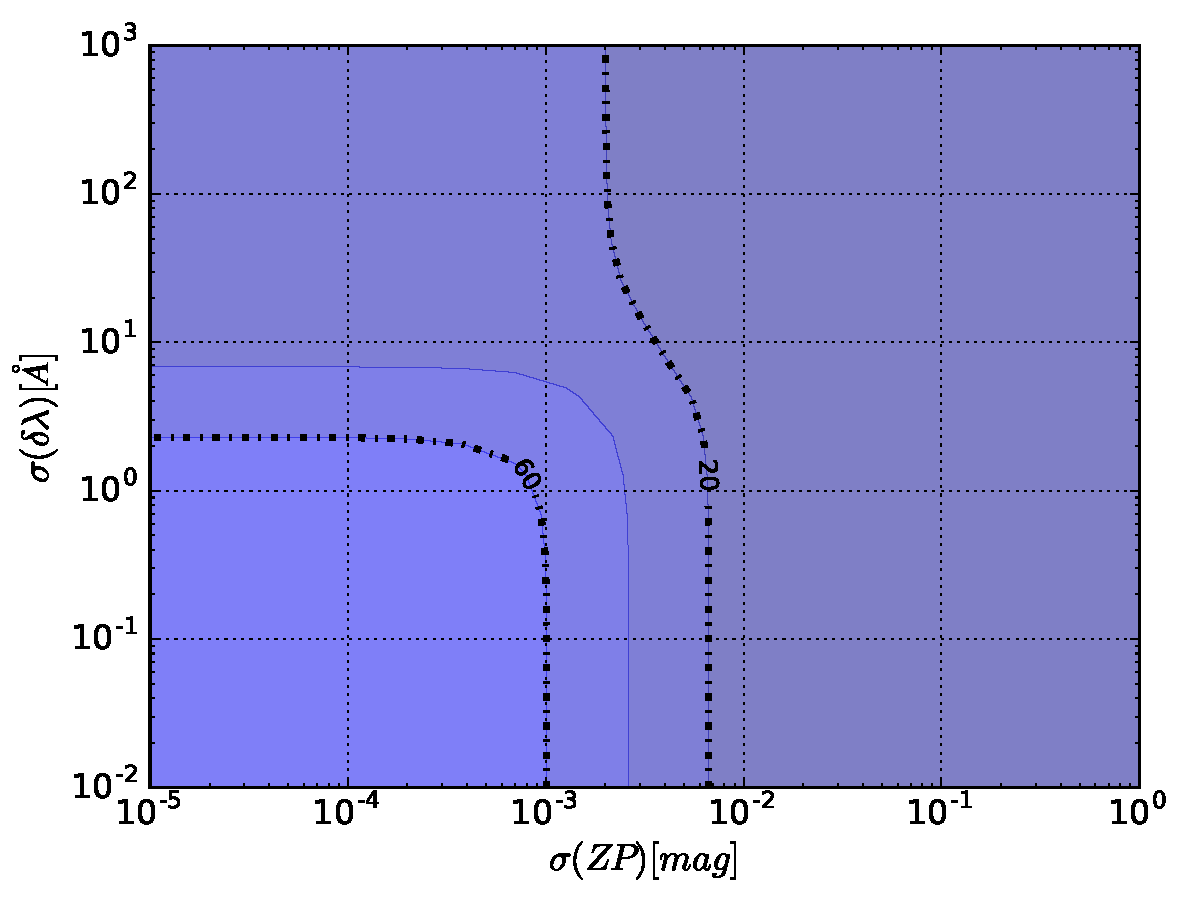
\includegraphics[width=0.48\linewidth]{FoM-grid_1-seasons_AltSched_with-training.pdf}}
\subfigure[5 years]{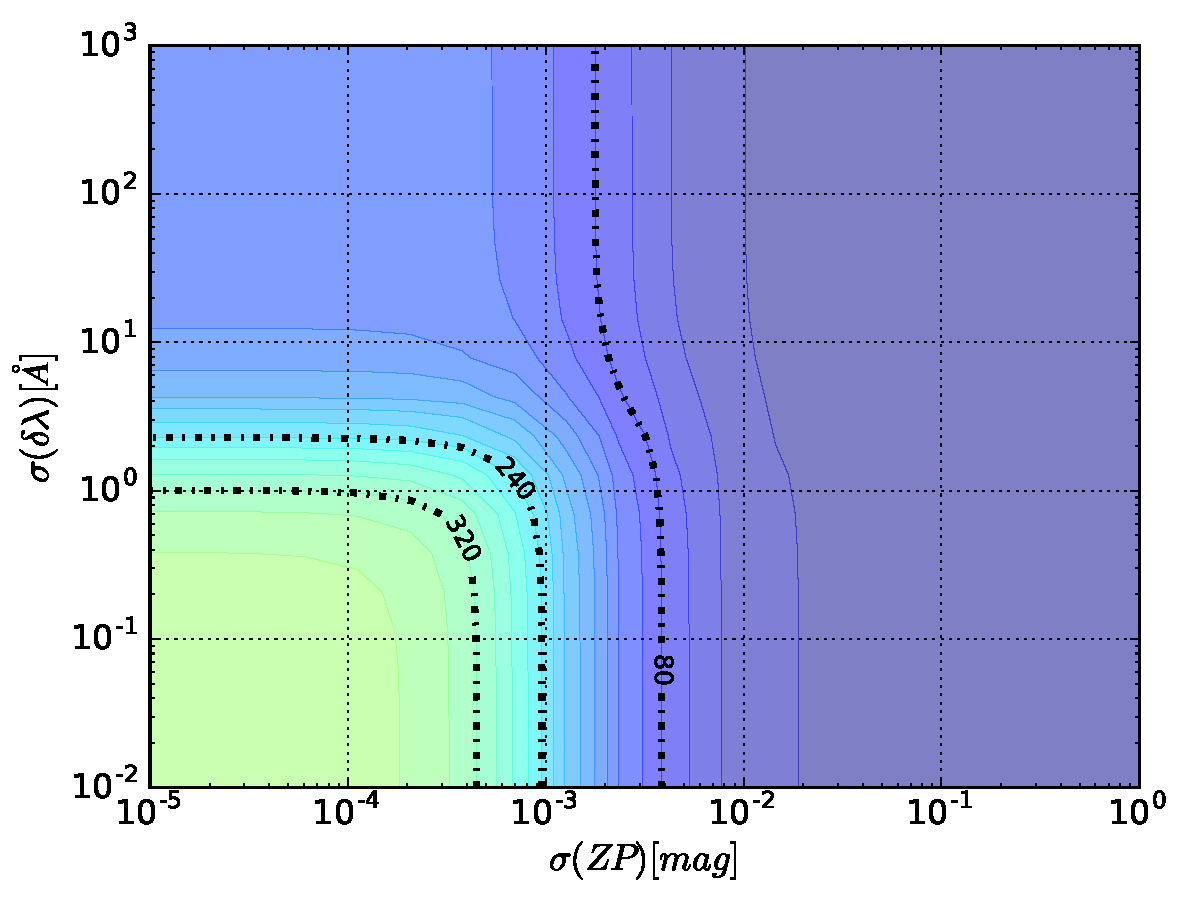
\includegraphics[width=0.48\linewidth]{FoM-grid_5-seasons_AltSched_with-training.pdf}}\\
\subfigure[10 years]{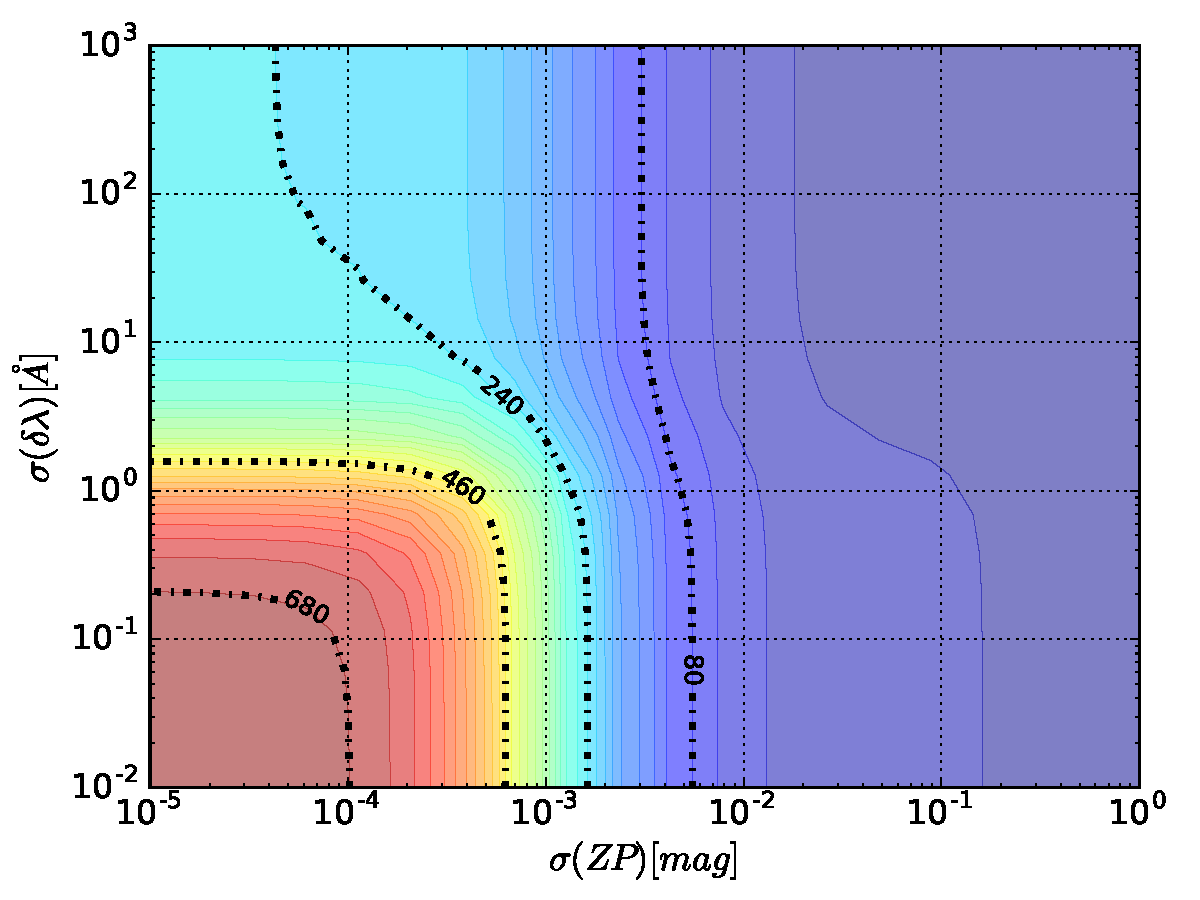
\includegraphics[width=0.48\linewidth]{FoM-grid_10-seasons_AltSched_with-training.pdf}}
\subfigure[10 years (slice)]{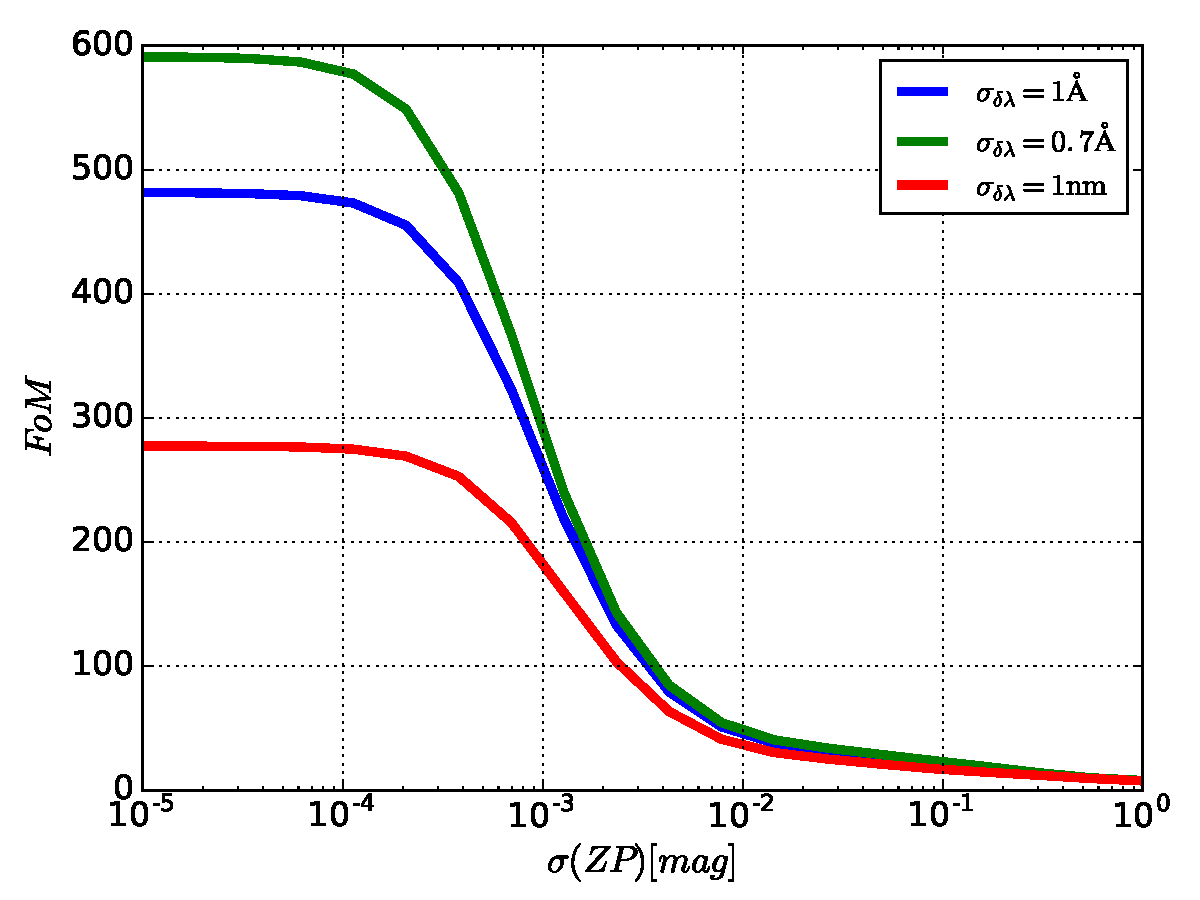
\includegraphics[width=0.48\linewidth]{FoM-plot_10-years.pdf}}
\caption{ (a), (b) \& (c) : FoM that can be achieved at one, five and
  ten years (full SN-survey). The FoM iso-countous are represented on
  a same color base for the 3 plots. Indicative iso-contours are
  represented in dot-dashed lines at some given FoM. The x-axis
  represents the a priori uncertainty on the filters zeropoint while
  the y-axis represents the uncertainty on the mean filter
  position. Each small iso-contour is separated from the others by 20
  points in the FoM. \\ (d) : Slices of (c) at
  $\sigma_{\delta\lambda} = 1\mathrm{\AA}$ in
  blue, $\sigma_{\delta\lambda} = 0.7\mathrm{\AA}$ in green and
  $\sigma_{\delta\lambda} = 1\mathrm{nm}$ in red.}
\label{fig:fom_grids}
\end{center}
\end{figure*}


% ----------------------------------------------------------------------

\section{Discussion}
\label{sec::discussion}
\subsection{Impact of the model training}
\label{ssec::training}
As a parallel work, we wanted to study what would be this result without the training of our spectrophotometric model, that is by not considering $\theta_P$ as free parameters.
Figure \ref{fig:fom_wout_training} shows that, compared to what we obtain with the training, we are making a large overestimation of the performances of the survey, that goes along with an underestimation of the impact of photometric calibration.
\begin{figure}[ht]
  \centering
  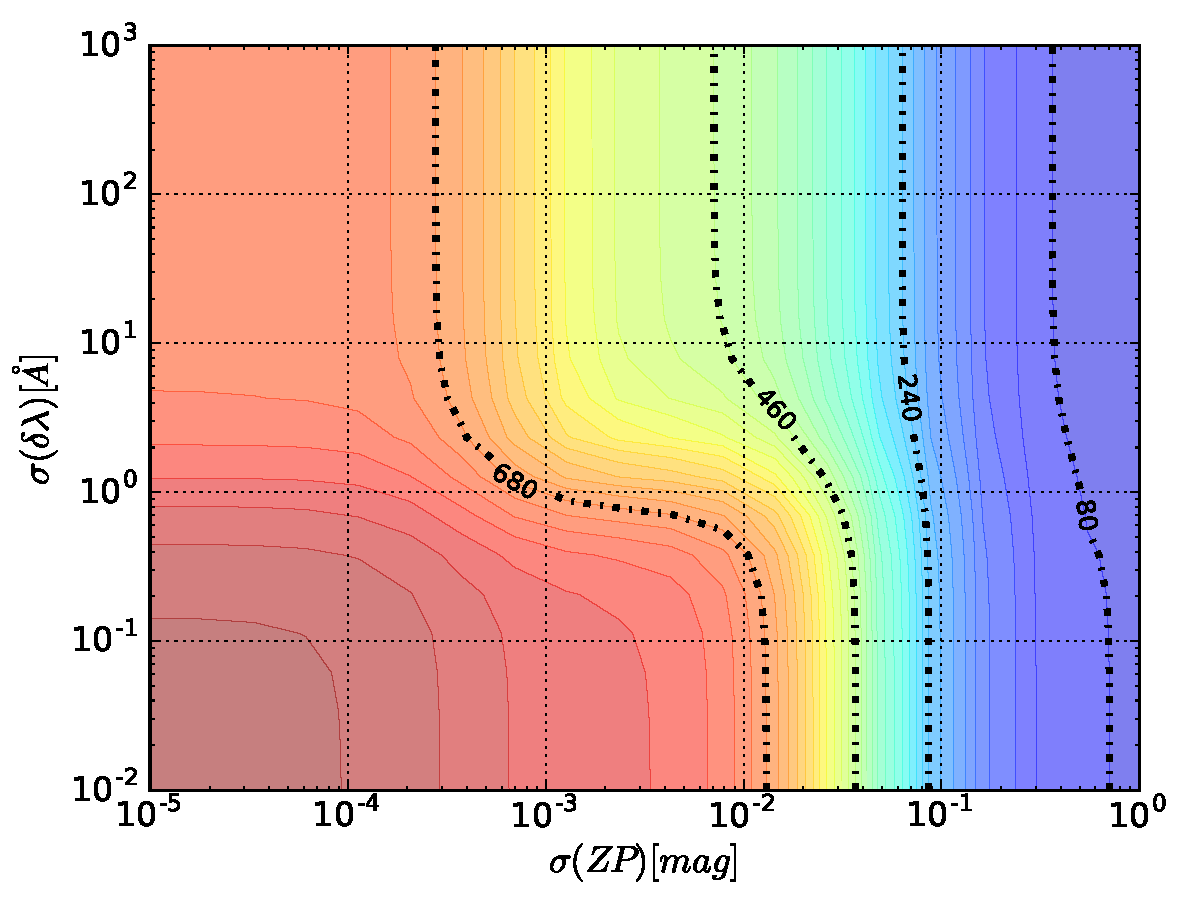
\includegraphics[width=\linewidth]{FoM-grid_10-seasons_AltSched_no-training.pdf}
  \caption{Evolution of the $FoM$ with respect to the filte position
    uncertainty and the filter zeropoint as in Figure
    \ref{fig:fom_grids} but without training the spectrophotometric
    model.}
  \label{fig:fom_wout_training}
\end{figure}
We can also notice that the $FoM$ is different from 0 even when the knowledge on the zero-points is minimal.
This auto-calibration of the zero-points is an artifact assuming a perfectly calibrated SN model.

\subsection{Filter position auto calibration}
As has been said in section \ref{sec::results}, the $FoM$ does not
fall to zero with a dramatical decrease of the accuracy on the filter
mean position, this seems to occur because of an auto-calibration
phenomenon.  We have added the spectral diversity of the type Ia SNe
as a pedestal on the uncertainty of the flux measured for each SN in
each band, which weakened the auto-calibration.  Caution should be
exercised before concluding that such an autocalibration of filter
passband could occur in the analysis of actual data:
\begin{itemize}
\item we assume a perfectly known redshift.
\item there is no high frequency spectral features in our photometric SN model
\item We use a simple parametrization of the filter uncertainties
\end{itemize}
Since we can already spot the transition area where a small
improvement in the filter position calibration leads to a great
improvement of the performances, this work still give us the main
information on the requirements we should reach. A later version of
this work will take into account these cautions


% We can notice that, assuming a smooth cosmology, there does not seem to be degeneracies between the filter positions and cosmological parameters.
% This is because filter shifts introduce wiggles in the Hubble Diagram (see Figure \ref{fig:lambda_der}) that can be spotted and erased by the fit.

% ----------------------------------------------------------------------

\section{Conclusion}
\label{sec::conclusions}

We show in this study that we can expose a relation between the
calibration parameter uncertainties and the performances of a LSST SN
survey by using a model fitting simultaneously the spectrophotometric
evolution of the SNe Ia, the cosmology and the calibration parameters.
We have also shown the necessity to take into account the training of
the spectrophotometric model over the dataset to obtain realistic
results from this type of study.  The exposed relation highlights the
necessity to calibrate the throughput of the LSST filters with a
precision better than $10^{-3}$ level in order to exploit at a good
level the increase of statistics that LSST will bring.  Finaly we
found that the uncertainty on the filters positions seem to have a
lesser effect on the performances.  We explain this phenomenon by the
fact that we are fitting together a smooth cosmology and the SN
spectrophotometric model, and the fact that the size and the quality
of the SN sample we have simulated is very high.  This particular
point will be investigated in a second iteration of this work, in a
first time by adding an uncertainty on the redshift of each SN
allowing for spatial inhomogeneities of filter passbands and in a
second time by adding the phase dimension of the spectrophotometric
evolution of the SNe Ia. We can finally see that we are in a good
agreement with the DESC SRD v0.9 concerning the calibration
requirements.


% ----------------------------------------------------------------------

\subsection*{Acknowledgments}

%Here is where you should add your specific acknowledgments, remembering that some standard thanks will be added via the \code{acknowledgments.tex} and \code{contributions.tex} files.

%% 
This is the text imported from \code{acknowledgments.tex}, and will be replaced by some standard LSST DESC boilerplate at some point.
% 


\input{contributions}

%{\it Facilities:} \facility{LSST}

% Include both collaboration papers and external citations:
\bibliography{lsstdesc,main}

\end{document}
% ======================================================================
% 
